\documentclass[a4paper,12pt]{article}
\usepackage{amsmath}
\usepackage{amssymb}
\usepackage[polish]{babel}
\usepackage{polski}
\usepackage[utf8]{inputenc}
\usepackage{indentfirst}
\usepackage{geometry}
\usepackage{array}
\usepackage[pdftex]{color,graphicx}
\usepackage{subfigure}
\usepackage{afterpage}
\usepackage{setspace}
\usepackage{color}
\usepackage{wrapfig}
\usepackage{listings}
\usepackage{datetime}
\usepackage[outdir=./]{epstopdf}

\renewcommand{\onehalfspacing}{\setstretch{1.6}}

\geometry{tmargin=2.5cm,bmargin=2.5cm,lmargin=2.5cm,rmargin=2.5cm}
\setlength{\parindent}{1cm}
\setlength{\parskip}{0mm}

\newenvironment{lista}{
\begin{itemize}
  \setlength{\itemsep}{1pt}
  \setlength{\parskip}{0pt}
  \setlength{\parsep}{0pt}
}{\end{itemize}}

\newcommand{\linia}{\rule{\linewidth}{0.4mm}}

\definecolor{lbcolor}{rgb}{0.95,0.95,0.95}
\lstset{
    backgroundcolor=\color{lbcolor},
    tabsize=4,
  language=C++,
  captionpos=b,
  tabsize=3,
  frame=lines,
  numbers=left,
  numberstyle=\tiny,
  numbersep=5pt,
  breaklines=true,
  showstringspaces=false,
  basicstyle=\footnotesize,
  identifierstyle=\color{magenta},
  keywordstyle=\color[rgb]{0,0,1},
  commentstyle=\color{Darkgreen},
  stringstyle=\color{red}
  }

\begin{document}

\noindent
\begin{tabular}{|c|p{11cm}|c|} \hline 
Grupa 1 & Kordian Kurdziel, Mateusz Maciejak & \ddmmyyyydate\today \tabularnewline
\hline 
\end{tabular}


\section*{Zadanie 4 - Liczby pierwsze - OpenMP}

Celem programu był test czy liczby podane w pliku są liczbami pierwszymi. W celu poprawy wydajności obliczeń program należało zrównoleglić z użyciem standardu OpenMP.

Program przyjmuje na wejściu dwa argumenty: liczbę wątków oraz ścieżkę do pliku w którym znajdują się liczby do przetestowania. Pierwszą rzeczą jaką wykonuje program jest sprawdzenie czy została podana odpowiednia ilość argumentów. Następnie zostaje wczytany plik a wpisane liczby umieszczone są w tablicy.
\begin{lstlisting}
    #pragma omp parallel for default(none) shared(results, numbersFromFileArr) private(i) schedule(dynamic) num_threads(numberOfThreads)
    for (i = 0 ; i < sizeof(numbersFromFileArr)/sizeof(*numbersFromFileArr) ; i++) {
        if (isPrime(numbersFromFileArr[i])){
            results[i] = true;
        } else {
            results[i] = false;
        }
    }
\end{lstlisting}

Powyższy fragment kodu zrównolegla działania wykonywane w pętli. Dyrektywa zrównoleglania została ustawiona na wartość default. W klauzuli shared została umieszczona tablica przechowująca wynik oszacowania czy liczba jest pierwsza oraz tablica zawierająca liczby z plików. 
Jako zmienna prywatna została ustalona wartość licznika pętli. Klauzula schedule została ustalona na wartość dynamic, gdyż w takiej konfiguracji udało się pozyskać najbardziej optymalne wyniki.

\begin{lstlisting}
bool isPrime(ll n)
{
    if(n<2)
        return false;
        
    for(ll i=2;i*i<=n;i++)
        if(n%i==0)
            return false; 

    return true;
}

\end{lstlisting}

Powyższy listing przedstawia algorytm wyznaczania liczby pierwszej. Został wybrany algorytm naiwny, ponieważ gwarantował poprawność wyników, a ilość i długość testowanych liczb nie była na tyle długa by powodowało to znaczące obniżenie wydajności obliczeń. 
W poszczególnych wątkach sprawdzane jest czy dana liczba jest liczbą pierwszą. Dane zostają podzielone na części i obliczane równolegle, używając wewnętrznych kopii danych w wątku.

Poniższe wykresy przedstawiają wyniki uzyskane na serwerze CUDA. Pierwszy wykres przedstawia zależność czasu obliczeń od liczby wątków. Drugi wykres przedstawia wartość przyspieszenia obliczeń względem programu uruchamianego synchronicznie w zależnośći od liczby wątków.

\begin{figure}[!ht]
	\centering
  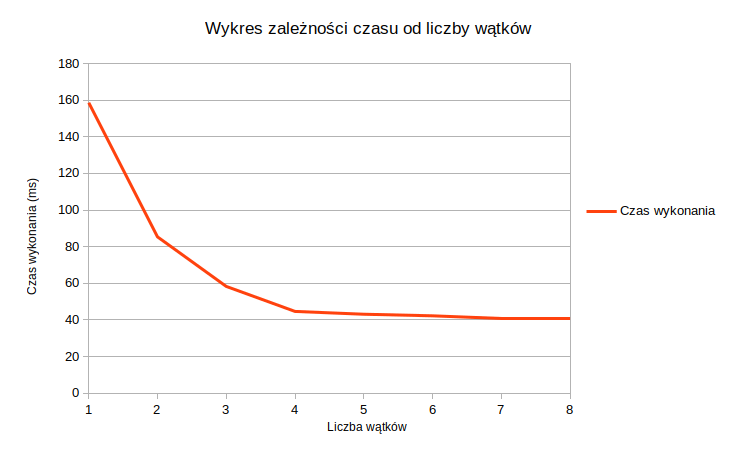
\includegraphics[width=0.9\textwidth]{wykresCzas.png}
  \caption{Wykres zależności czasu wykonywania obliczeń od liczby wątków}
\end{figure}

\begin{figure}[!ht]
	\centering
  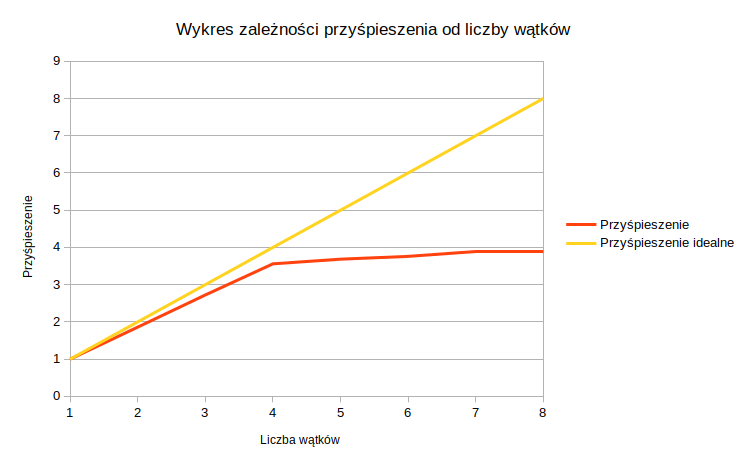
\includegraphics[width=0.9\textwidth]{wykresPrzyspieszenie.png}
  \caption{Wykres przyspieszenia działania programu w zależności od liczby wątków}
\end{figure}


Jak można zauważyć, program przyśpiesza aż do osiągnięcia granicy 4 wątków. Dzieje się tak, gdyż procesor na którym program został uruchomiony posiada 4 rdzenie oraz korzysta z technologii \quotedblbase Hyper-Threading\textquotedblright.
Dzięki wykorzystaniu technologii OpenMP udało się uzyskać przyśpieszenie bliskie idealnemu, co świadczy o tym że przedstawione obliczenia dobrze nadają się do zrównoleglenia.

\end{document}
